\documentclass{article}

\usepackage{graphicx}
\usepackage{tikz}
\usepackage{tikzsymbols}
\usetikzlibrary{calc,patterns,shapes.geometric}
\pagestyle{empty}
\usepackage[margin=0pt]{geometry}
\geometry{papersize={14in,12in}}

\def\centerarc[#1](#2)(#3:#4:#5){\draw[#1] ($(#2)+({#5*cos(#3)},{#5*sin(#3)})$) arc (#3:#4:#5);}

\begin{document}
	\begin{figure}
		\centering
		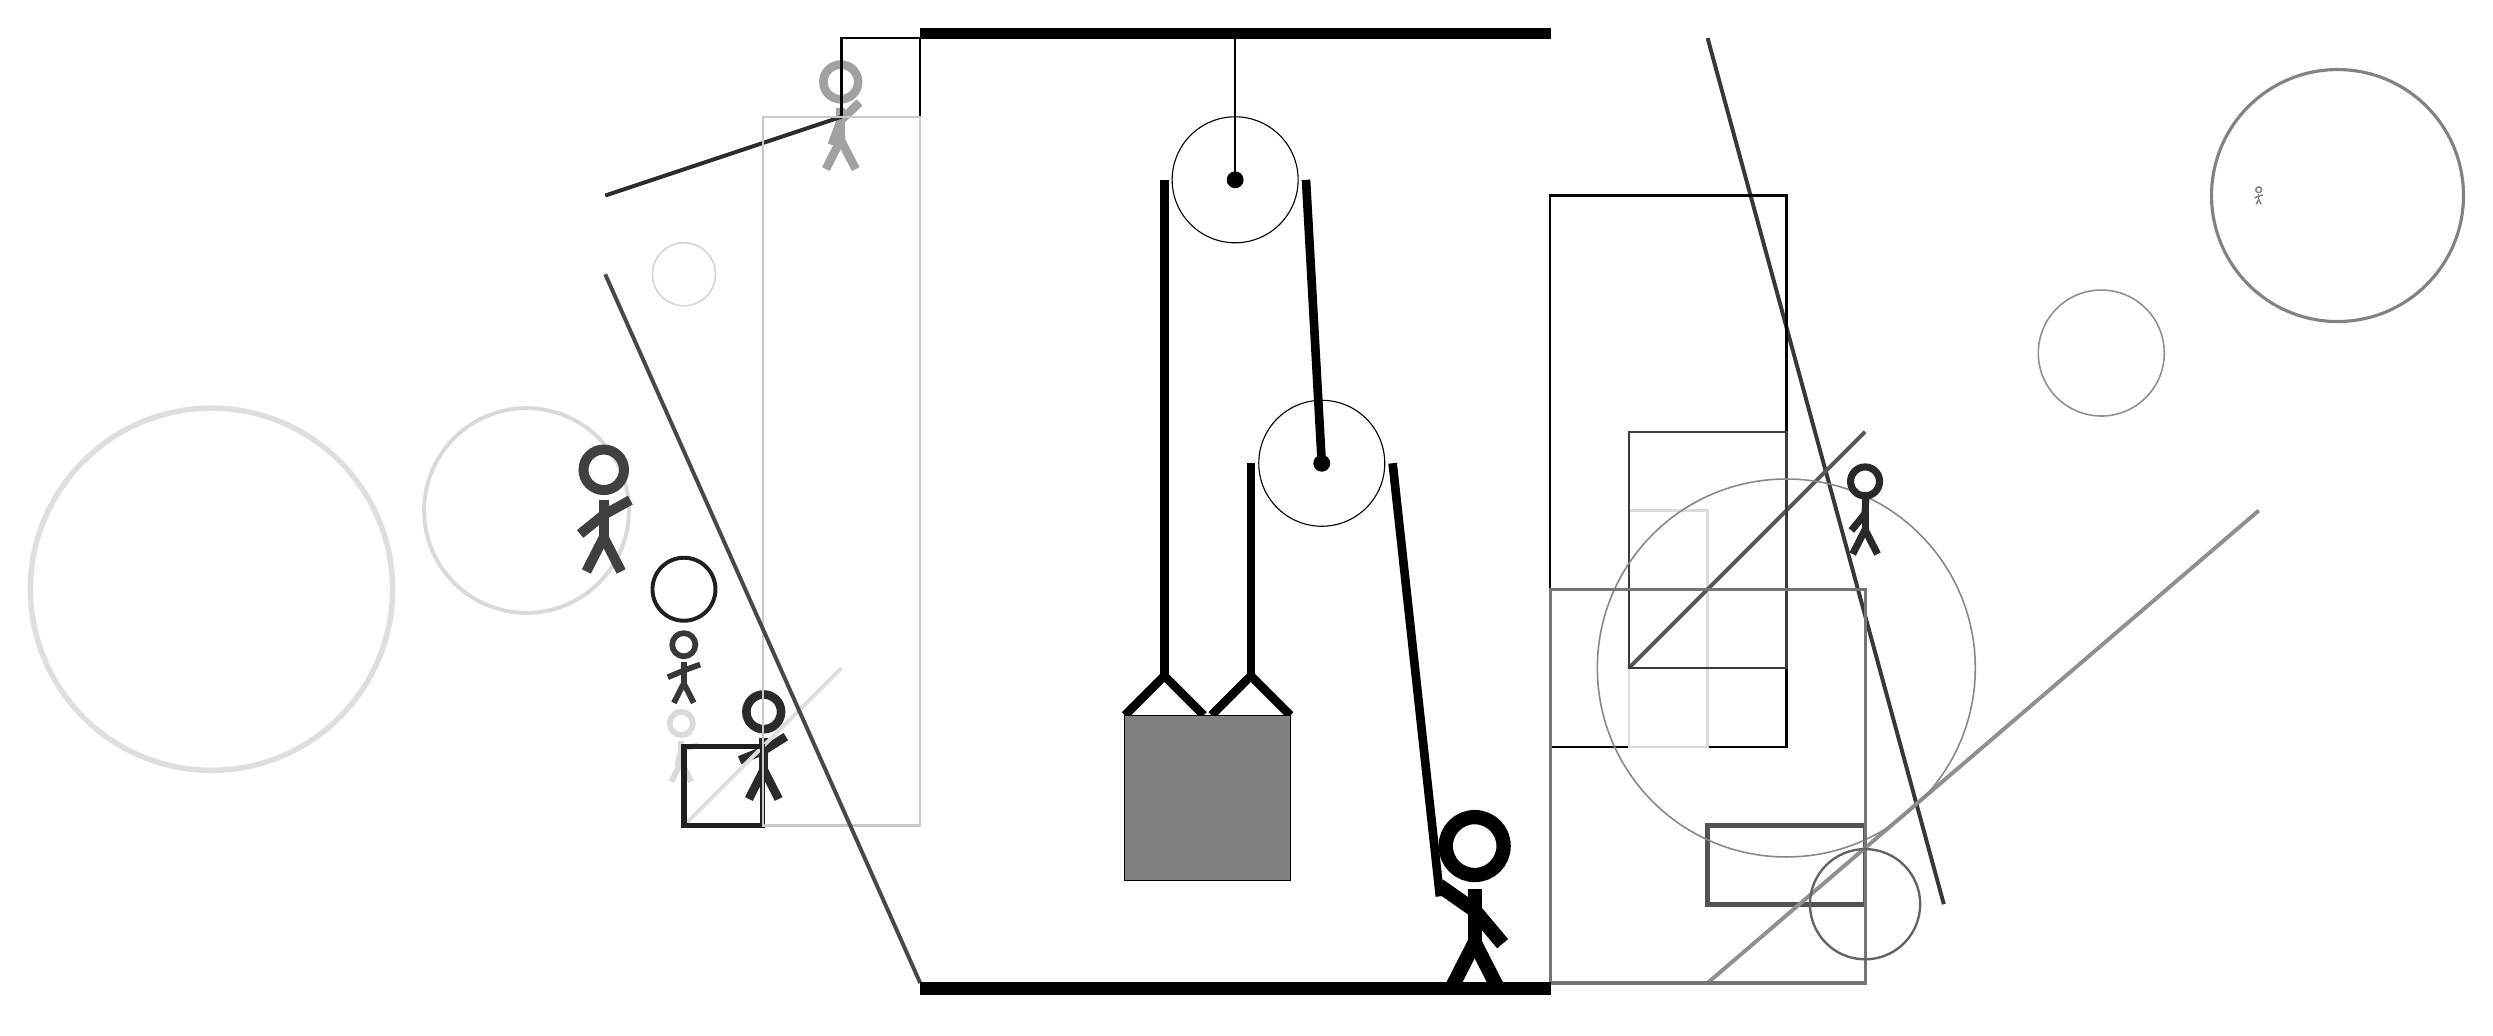
\begin{tikzpicture}
			%%%%% START %%%%%
			
			\draw[fill=black] (-2, 9) rectangle (6, 9.125);
			
			\draw (2, 7.2) circle (0.8);
			\draw[fill=black] (2, 7.2) circle (0.1);
			\draw[thick] (2, 7.2) -- (2, 9);
			
			\draw (3.1, 3.6) circle (0.8);
			\draw[fill=black] (3.1, 3.6) circle (0.1);
			
			\node[line width=0.6mm, color=black!83] at (-4, 0) {\Strichmaxerl[6][22][32]};
			
			\node[line width=0.4mm, color=black!37] at (-3, 8) {\Strichmaxerl[6][70][44]};
			\draw[line width=0.3mm, color=black!99] (-2, 9) rectangle (-3, 8);
			\draw[line width=0.5mm, color=black!83](-3, 8) -- (-6, 7);
			
			\draw [line width=0.2mm, color=black!44](13, 5) circle (0.8);
			\draw[line width=0.5mm, color=black!78](8, 9) -- (11, -2);
			
			\draw[line width=0.6mm, color=black!68] (8, -2) rectangle (10, -1);
			\draw[line width=0.3mm, color=black!100] (6, 7) rectangle (9, 0);
			\node[line width=0.6mm, color=black!51] at (15, 7) {\Strichmaxerl[1][23][15]};
			\draw[line width=0.3mm, color=black!14] (8, 3) rectangle (7, 0);
			\draw[line width=0.5mm, color=black!13](-5, -1) -- (-3, 1);
			
			\node[line width=0.5mm, color=black!78] at (-5, 1) {\Strichmaxerl[4][23][20]};
			\draw[line width=0.5mm, color=black!66](10, 4) -- (7, 1);
			
			\node[line width=0.6mm, color=black!15] at (-5, 0) {\Strichmaxerl[4][76][13]};
			\draw[line width=0.5mm, color=black!44](8, -3) -- (15, 3);
			\draw[line width=0.3mm, color=black!77] (7, 4) rectangle (9, 1);
			
			\draw [line width=0.5mm, color=black!15](-7, 3) circle (1.3);
			
			\draw [line width=0.5mm, color=black!88](-5, 2) circle (0.4);
			\draw [line width=0.2mm, color=black!47](9, 1) circle (2.4);
			\draw[line width=0.7mm, color=black!88] (-4, 0) rectangle (-5, -1);
			\node[line width=0.7mm, color=black!84] at (10, 3) {\Strichmaxerl[5][51][87]};
			\draw[line width=0.3mm, color=black!21] (-2, -1) rectangle (-4, 8);
			\draw[line width=0.4mm, color=black!54] (6, 2) rectangle (10, -3);
			\draw [line width=0.2mm, color=black!17](-5, 6) circle (0.4);
			\draw [line width=0.3mm, color=black!61](10, -2) circle (0.7);
			
			\draw [line width=0.4mm, color=black!49](16, 7) circle (1.6);
			\node[line width=0.6mm, color=black!75] at (-6, 3) {\Strichmaxerl[7][39][29]};
			\draw [line width=0.7mm, color=black!13](-11, 2) circle (2.3);
			
			\draw[line width=0.5mm, color=black!72](-2, -3) -- (-6, 6);
			
			
			\draw[line width = 1.1mm]  (0.6, 0.4) -- (1.1, 0.9) -- (1.6, 0.4);
			\draw[line width = 1.1mm]  (1.7, 0.4) -- (2.2, 0.9) -- (2.7, 0.4);
			\draw[fill=black!50] (0.6, 0.4) rectangle (2.7, -1.7);
			
			\draw[line width = 1.1mm] (1.1, 7.2) -- (1.1, 0.9);
			\centerarc[line width = 1.1mm](2, 7.2)(0:180:0.9);
			\draw[line width = 1.1mm] (2.9, 7.2) -- (3.1, 3.6);
			\draw[line width = 1.1mm] (2.2, 3.6) -- (2.2, 0.9);
			\centerarc[line width = 1.1mm](3.1, 3.6)(0:180:0.9);
			\draw[line width = 1.1mm] (4.0, 3.6) -- (4.6, -1.9);
			
			\node at (5, -2) {\Strichmaxerl[10][-35][-50]};
			
			\draw[fill=black] (-2, -3) rectangle (6, -3.15);
			
			%%%%% END %%%%%
		\end{tikzpicture}
	\end{figure}	
\end{document}